\section{Validation}

Cette partie vise à tester et valider le comportement des blocs fonctionnels.
Elle se positionne sur la pente remontante du cycle en V.
Comme le détaille, J.P. Calvez dans \textit{Spécification et conception des systèmes - une méthodologie} \cite{Calvez_2}, la seconde moitié du cycle commence par les éléments élémentaires pour remonter progressivement jusqu'au produit complet.
\begin{figure}[H]
    \centering
    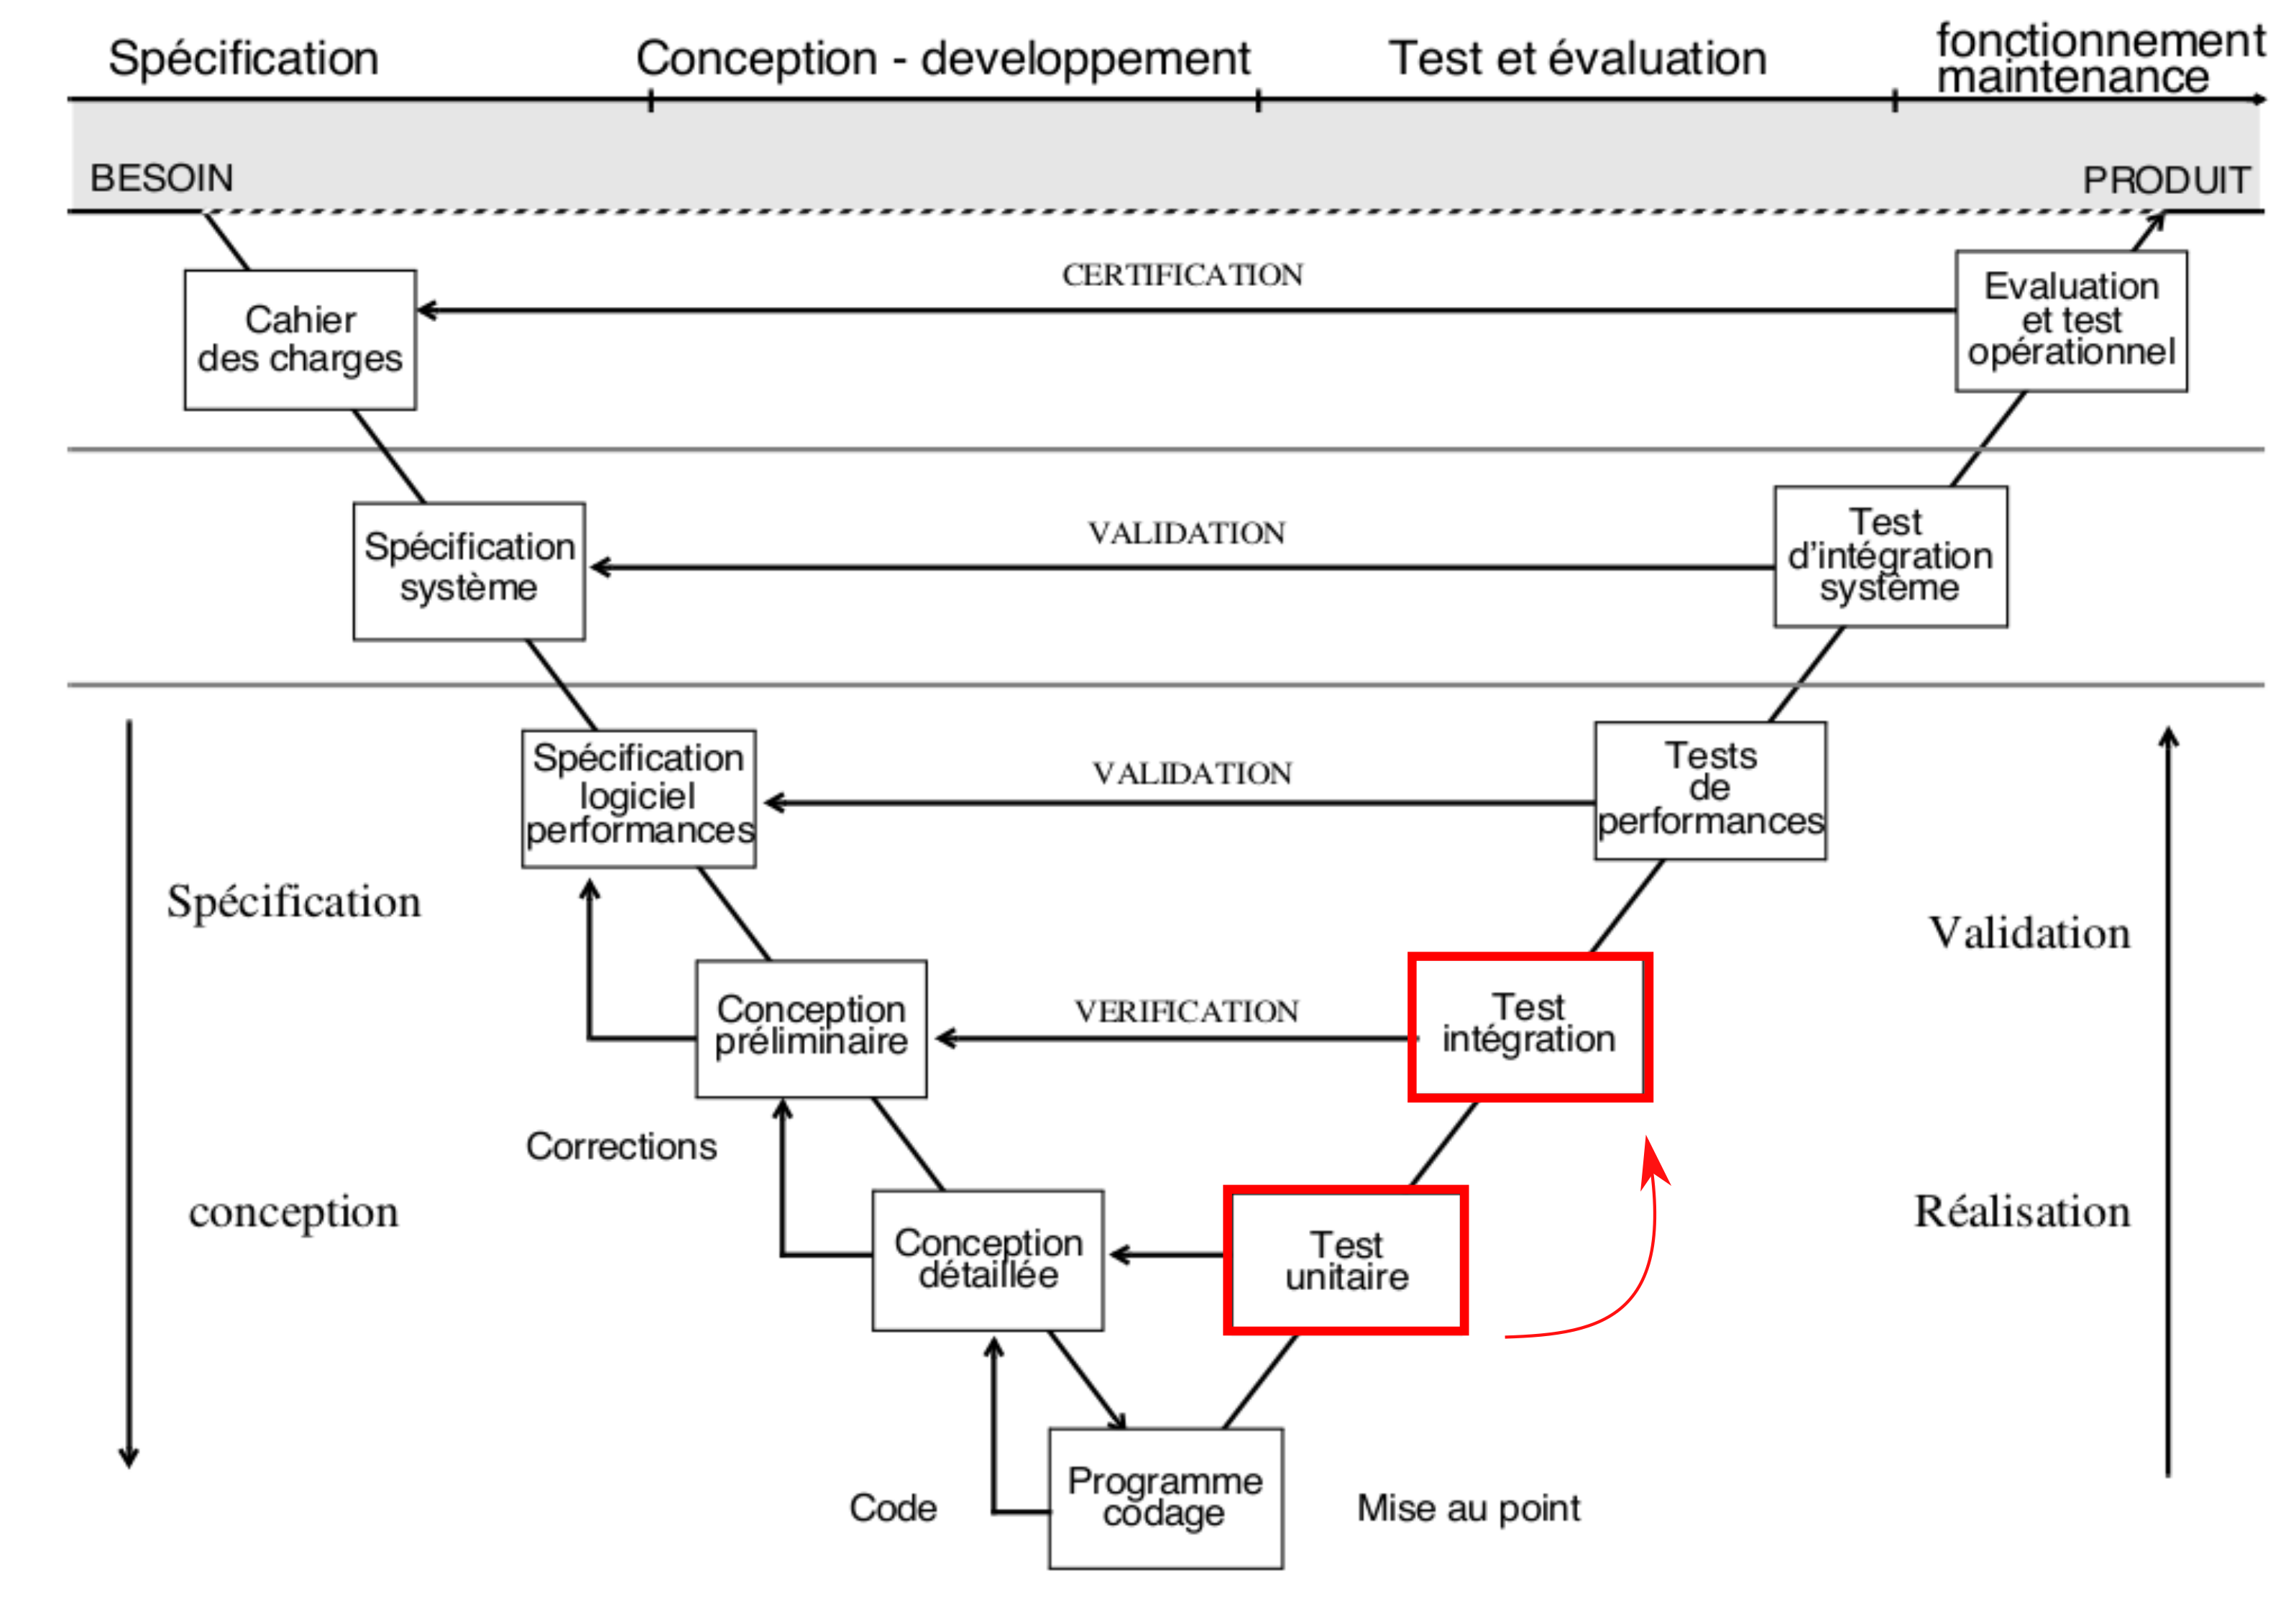
\includegraphics[width=0.8\linewidth]{cycle_V_validation.draw.png}
    \caption{Exemple de cycle en V }
    \label{fig:cycle_v}
\end{figure}
Dans un premier temps une attention particulière sera portée à vérifier le bon fonctionnement des blocs élémentaires de notre conception détaillée. 
Dans un second, un test plus proche des conditions d'utilisation se focalisera sur le périphérique avec toutes les entités intégrées.
N'ayant aucune information sur la technologie à utiliser dans le cahier des charges, ce rapport se contentera de ces deux phases de test. 
En effet, il n'est pas possible de réaliser la partie test de performance où intégration système.

\subsection{Test unitaire}
Le test unitaire vise à isoler chaque bloc unitaire afin de vérifier son fonctionnement.
Le comportement des blocs adjacents est alors simulé par le testbench.
Dans ce contexte, il est possible de moduler les signaux d'entrée de manière plus flexible.
Il serait naïf pour un ingénieur débutant de négliger cette étape en passant directement à la phase d'intégration.
En effet, elle permet d'identifier un certain nombre d'erreurs et de les résoudre dans un environnement de test simplifié.
Dans un cadre industriel cela permet de limiter les coûts d'intégration \cite{Calvez_2}.
\subsubsection{Solutionneur de priorités}
Le bloc solutionneur de priorités prend en entrée les 15 sources d'interruptions provenant des autres périphériques et le registre des priorités.
Il doit, à partir de cela, présenter en sortie le numéro de l'interruption active la plus prioritaire.
La gestion des interruptions n'étant pertinente, dans un processeur, que si la latence est réduite au minimum.
C'est pourquoi nous avons fait le choix de concevoir une solution asynchrone qui assure sa fonction en moins d'un cycle horloge.
La simulation suivante ne possède donc pas d'horloge.
Les deux conditions de priorité sont testées.
La première, si deux interruptions sont valides au même instant, c'est l'identifiant de la plus prioritaire au regard du registre \texttt{CTRL\_IT\_PRIO\_N} qui est placé en sortie.
La seconde, correspond au cas particulier où deux interruptions de même priorité seraient actives simultanément.
Dans cette situation, c'est l'identifiant le plus grand qui est sélectionné.
\begin{figure}[H]
    \centering
    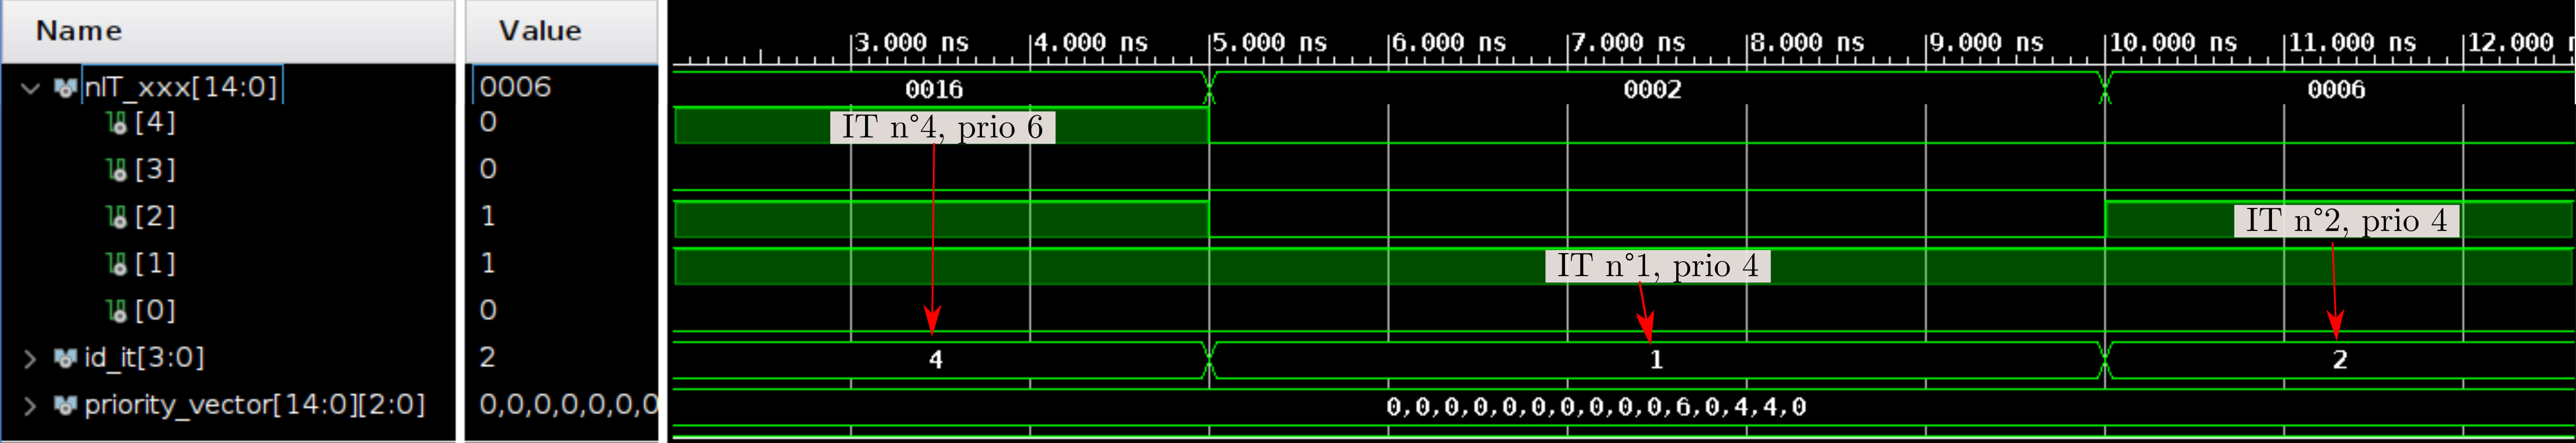
\includegraphics[width=1.1\linewidth]{chrono_priority_solver.draw.png}
    \caption{Chronogramme validation solutionneur priorité}
    \label{fig:chrono_prio_solv}
\end{figure}
La figure \ref{fig:chrono_prio_solv} illustre le résultat du bloc solutionneur priorité lorsqu'il est soumis à une banc de test.
Bien que les stimulus d'entrée prennent un grand nombre de valeurs dans la simulation originale, seul trois cas sont présentés.
Les priorités sont inchangées au cours de ce test et leur valeur sont $IT_4=6$, $IT_1=4$, $IT_2=4$.
Dans le premier, trois interruptions sont valides simultanément.
C'est l'identifiant 4 qui est placé en sortie, car sa priorité est de 6 contre 4 pour deux les autres.
Dans le deuxième cas, seul une interruption est valide, il n'y a pas d'arbitrage, la valeur 1 est visible en sortie.
Le dernier illustre la situation particulière où les 1 et 2 ont la même priorité.
C'est donc le numéro 2 qui prend la main.
Le chronogramme atteste du bon fonctionnement du bloc solutionneur de priorités.


\subsubsection{Masque}

Le bloc masque permet à l'utilisateur d'inhiber les sources d'interruption de son choix.
Il prend en entrée les 15 sources d'interruption et le registre \texttt{CTRL\_IT\_MSQ}.
Son fonctionnement est plutôt simple.
Le registre est d'abord inversé bit à bit puis un ET logique est appliqué avec les sources.
Seuls, les bits non masqués sont transmis au bloc suivant.
\begin{figure}[H]
    \centering
    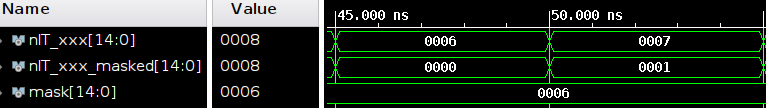
\includegraphics[width=0.8\linewidth]{chrono_mask.png}
    \caption{Chronogramme validation bloc masquage}
    \label{fig:chrono_mask}
\end{figure}
La figure \ref{fig:chrono_mask} illustre deux exemples du bloc masquage soumis aux stimulus du banc de test.
Le masque est affecté à la valeur 6, $(110)_2$, pendant les deux situations.
Les sources 1 et 2 sont donc  masquées.
Dans le premier cas, ces deux sources sont actives, elles sont donc inactivées sur la sortie.
Dans un second temps, la source 0 émet une demande d'interruption.
Cette dernière n'étant pas masqué, elle est conservée seule.



\subsubsection{Gestion branchement (blx)}

Le bloc gestion branchement est créé pour contrôler la temporalité des échanges avec le processeur de manière indirecte.
Il génère le signal \texttt{nIT\_CPU} et met à jour le registre de branchement au même instant.
Il garantit la validité de sa valeur, en empêchent les réécritures tant que le processeur n'a pas confirmé la lecture.
Si cela n'était pas fait, lorsqu'une interruption surviendrait entre la lecture du LSB et du MSB, l'adresse de branchement serait corrompue.
Dans l'exemple présenté ci-dessous, deux interruptions surviennent de manière rapprochée.
On considère que la seconde est plus prioritaire que la première et doit donc l'interrompre.
Nous cherchons à monter que cela n'est fait qu'après la prise en compte de la première.
\begin{figure}[H]
    \centering
    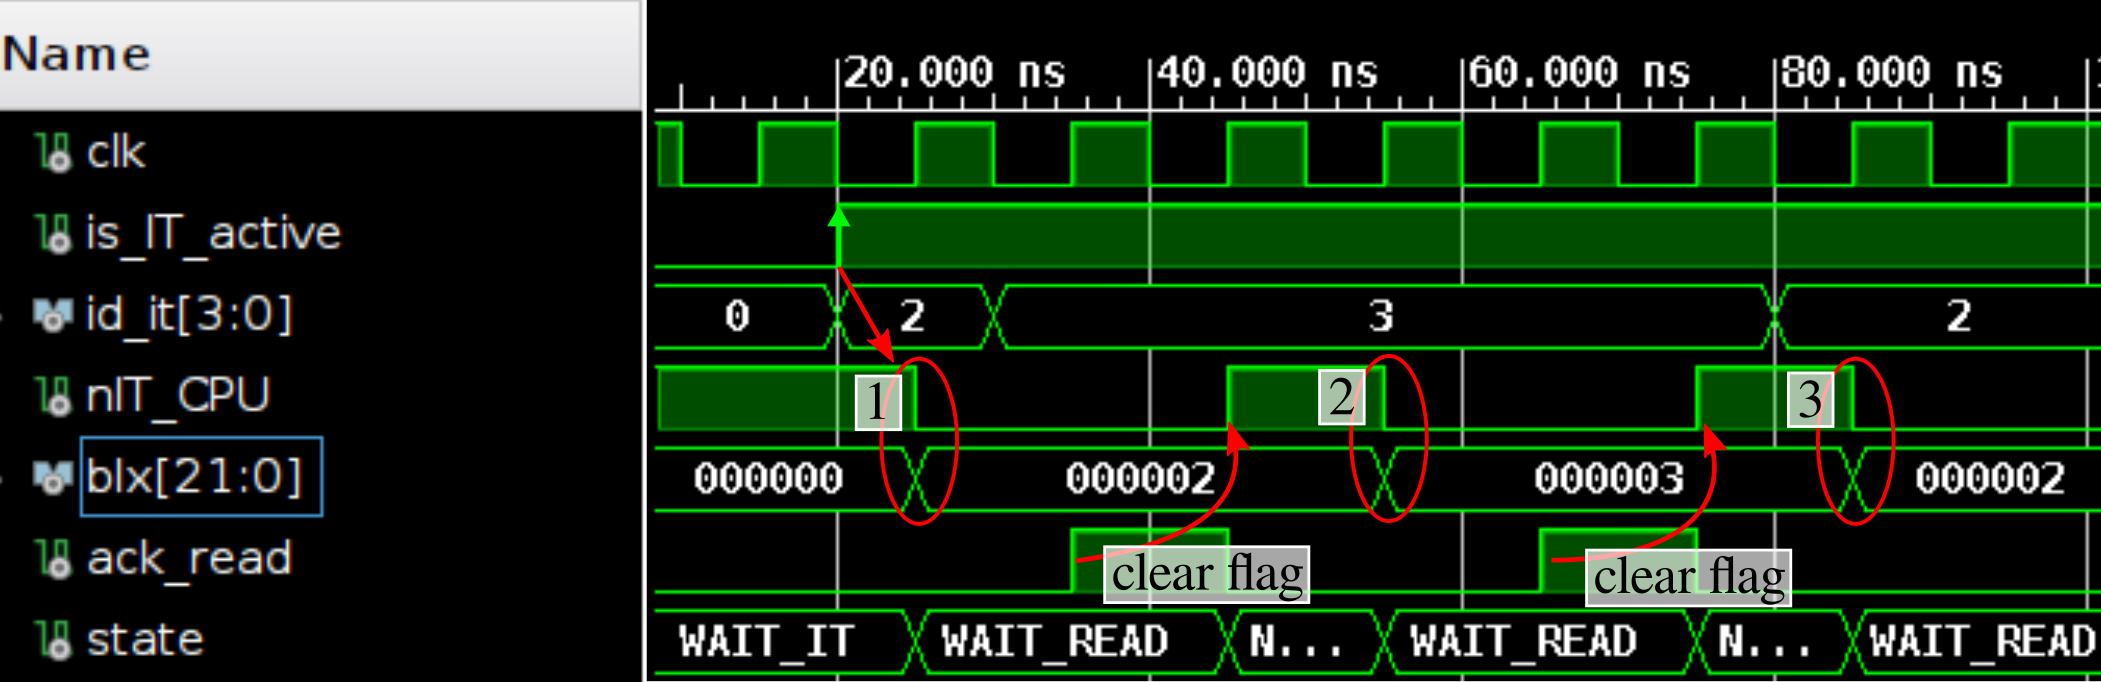
\includegraphics[width=0.8\linewidth]{chrono_gestion_blx.draw.png}
    \caption{Chronogramme validation bloc gestion branchement}
    \label{fig:chrono_blx}
\end{figure}
Le cas recherché est présenté figure \ref{fig:chrono_blx}.
Le passage de l'entrée \texttt{is\_IT\_active} à l'état haut indique qu'une donnée valide est présente sur \texttt{id\_IT} (cf [1]).
Le gestionnaire de branchement réagit en plaçant l'adresse de branchement dans le registre \texttt{@blx} et en assignant \texttt{nIT\_CPU} à 0.
Les adresses de branchement sont configurées avec le numéro de l'IT pour plus de lisibilité.
C'est pourquoi \texttt{@blx} vaut 2.
Un court moment après, \texttt{id\_IT} change de valeur, indiquant qu'une IT plus prioritaire survient.
Cela n'engendre aucune réaction, car l'interruption précédente n'a pas été acquittée.
Le processeur effectue une lecture dans le registre de branchement (LSB), le signal \texttt{ack\_read} passe à 1.
Pour rappel, \texttt{ack\_read} est généré par le bloc interface read.
Il y a bien eu acquittement, les données concernant la seconde interruption sont fournies (cf [2]).
On observe \texttt{@blx} = 3.
Ensuite, une nouvelle lecture est effectuée, on considère dans le testbench que l'interruption est traité en 1 coup d'horloge.
Le numéro d'interruption sur \texttt{id\_IT} repasse donc à 2 pour finir de traiter la première.
Le coup d'horloge suivant (cf [3]), l'adresse est placée dans le registre \texttt{@blx} et le CPU est informé via \texttt{id\_IT}.

\subsection{Test intégration}
Les tests unitaires viennent d'être présentés. 
Comme présenté dans l'introduction de la validation, la prochaine étape selon le cycle en V (figure \ref{fig:cycle_v}) est le test d'intégration.
Il vise à rassembler les blocs fonctionnels tester dans la partie précédente dans une même entité.
On veillera à les interconnecter suivant le résultat de la phase de conception.

\subsubsection{Configuration}
L'objectif de ce test est de simuler le comportement du processeur lors de la configuration.
Deux périphériques sont activés, l'UART et le PCI.
Dans un premier temps, le périphérique est désactivé.
Puis les adresses de branchement sont configurées, l'une après l'autre.
L'organisation des registres permet d'écrire la priorité de deux interruptions adjacentes en même temps.
Nous exploitons donc cette possibilité dans cet exemple.
La priorité de l'UART est fixée à 3 et celle du PCI à 5.
Finalement, le périphérique est activé grâce au registre \texttt{Enable}.
\begin{lstlisting}[style=CStyle]
void CTRL_IT_Config(void){
    /* Disable CTRL IT */
    CTRL_IT->CTRL_IT_EN = 0x0000;
    /* Set handler addr UART */
    CTRL_IT->CTRL_IT_ADDR[nIT_UART] = &UART_Handler;
    /* Set handler addr PCI */
    CTRL_IT->CTRL_IT_ADDR[nIT_PCI] = &PCI_Handler;
    /* Set priority PCI = 5, UART = 3*/
    CTRL_IT->prio.[nIT_PCI] = (uint16_t)((0x3 << 8) | 0x5);
    /* Enable CTRL IT */
    CTRL_IT->CTRL_IT_EN = 0x0001;
}
\end{lstlisting}
Une fois le comportement souhaité établi, il convient de le traduire en VHDL pour le testbench.
Cette étape aboutie à une expansion importante du nombre de lignes.
C'est pourquoi on ne présente ici la conversion d'une seule ligne afin d'exposer la méthode.
La dernière ligne visant à activer le périphérique est choisie pour des raisons de simplicité.
\begin{lstlisting}[style=vhdl]
-- Enable CTRL IT
-- In C : CTRL_IT->CTRL_IT_EN = 0x0001;
RnW <= '0'; nAS = '0';
addr <= addr_EN;
d_bus <= (0 => '1', others => '0');
\end{lstlisting}
Le comportement souhaité, sous-entendu par la ligne en C, est l'écriture d'un 1 dans le registre \texttt{Enable}.
Les signaux de contrôle sont affectés de sorte à indiquer une écriture.
L'adresse du registre est placée sur le bus d'adresse.
Le bus de données est affecté à '1'.
Cet exemple plutôt simple présente la méthode.
La même démarche est mise en œuvre pour les autres lignes C.
Dans la mesure où la donnée à transmettre est plus petite ou égale à la taille du bus de données, les instructions peuvent se faire en un cycle horloge.
L'écriture des adresses de branchement sont donc faites en deux coups d'horloges.
Le chronogramme \ref{fig:chrono_config_globale} présente le comportement du processeur simulé par le testbench et le résultat du périphérique soumis à ces requêtes.
\begin{figure}[H]
    \centering
    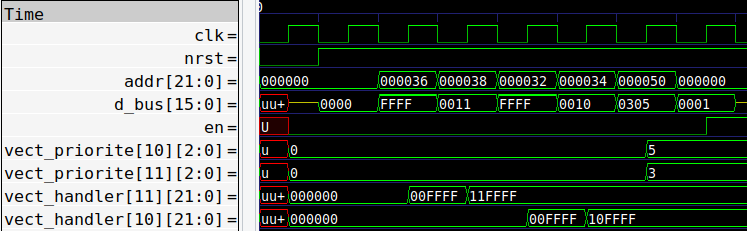
\includegraphics[width=0.75\linewidth]{config_globale.png}
    \caption{Chronogramme validation globale configuration}
    \label{fig:chrono_config_globale}
\end{figure}
On observe les 7 cycles d'écriture attendue, dans l'ordre suivant : \vspace*{-3mm}
\begin{itemize}
    \item CTRL\_IT\_EN \vspace*{-3mm}
    \item CTRL\_IT\_ADDR\_11 LSB \vspace*{-3mm}
    \item CTRL\_IT\_ADDR\_11 MSB \vspace*{-3mm}
    \item CTRL\_IT\_ADDR\_10 LSB \vspace*{-3mm}
    \item CTRL\_IT\_ADDR\_10 MSB \vspace*{-3mm}
    \item  CTRL\_IT\_PRIO\_10\_11
\end{itemize}
Nous cherchons à vérifier que les cycles d'écritures aboutissent tous en une valeur stocké dans un registre.
Cela est visible sur ce chronogramme.
Le fonctionnement de ce test en bien celui souhaité.
Par la même occasion, nous pouvons valider le bon fonctionnement du reset ayant lieu au début de la simulation.
Tous les registres affichés prennent la valeur 0.

\subsubsection{Interruptions simultanées}
Une fois la configuration du périphérique effectuée, il est possible de tester sa réaction à l'occurrence d'interruptions.
Nous choisissons de présenter un cas de complexité modérée.
Deux interruptions de priorité différentes apparaissent simultanément.
Le comportement attendu est le traitement de la plus prioritaire puis, après acquittement du CPU, la prise en charge de la seconde.
La figure \ref{fig:chrono_valide_globale_IT} présente le comportement du périphérique soumis à deux interruptions simultanées.
\begin{figure}[H]
    \centering
    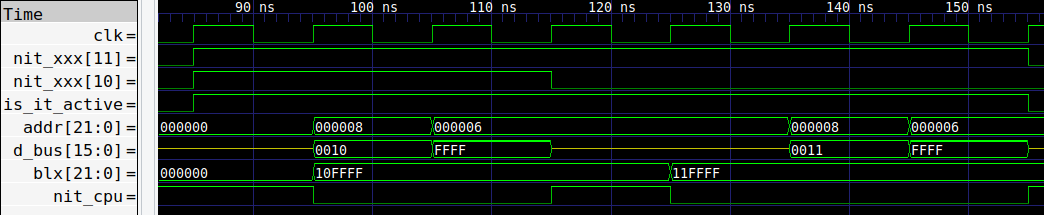
\includegraphics[width=\linewidth]{chrono_valide_globale_IT.png}
    \caption{Chronogramme validation globale interruptions simultanées}
    \label{fig:chrono_valide_globale_IT}
\end{figure}
Les signaux d'interruptions sont visibles au premier coup d'horloge.
Elles sont accompagnées du signal \texttt{is\_it\_active} qui comme son nom l'indique passe à haut si une interruption doit être traitée.
Le bloc gestion blx analyse, la requête fournie par le solutionneur de priorité et affecte la bonne valeur dans le registre de branchement en un cycle horloge.
La valeur est question est l'adresse de \texttt{PCI\_handler} que l'on reconnait par le préfixe 10 comme son numéro d'interruption.
Ce premier comportement satisfait nos attentes, c'est bien PCI la source la plus prioritaire.
Le CPU ayant été notifié par le signal \texttt{nIT\_CPU}, lit l'adresse de branchement.
Cela correspond à deux cycles horloge, le registre du LSB en interprété comme acquittement.
Il baisse ensuite la source d'interruption sur le périphérique émetteur.
L'interruption PCI est considérée comme complètement traitée à 125ns sur la figure \ref{fig:chrono_valide_globale_IT}.
À l'instant suivant (135ns), le processeur est notifié pour prendre en compte la seconde, initialement moins prioritaire.
Comme pour la première, l'adresse de branchement est placée dans le registre \texttt{blx}.
La lecture par le processeur prend deux cycles.
Toutes les interruptions sont traitées à 155ns, le signal \texttt{is\_it\_active} repasse à zéro.
Le fonctionnement du périphérique est validé par ce test ayant pour ambition de s'approcher au maximum d'un cas réel.
